% FIRST OF ALL:
% If you are using X-based Emacs to read this file, please switch on
% Syntax Highlighting by typing:
%    ALT-X  font-lock-mode   (or META-X on X-Terminals)
%
% That should make these comments nice and red so they can be easily
% distinguished from the actual code. 
% =======================================================================

% This is a template for Masters' Theses at WPI.
% It complies (more or less) to the standards given by the Library 
% (as of February 1999)
%
% Feel free to use this file, but I give no guarantee for its compliance
% to standards (meaning I won't pay for the paper if the library rejects it :))
%
%
% The lengths (textheight, width etc.) are fine-tuned for ps1, ps2, and ps3, 
% but seem to be somewhat dependent on the machine you are using to compile, 
% the date, time, moon phase, the weather, and other quantum effects.
% You may have to change \oddsidemargin a little, but it's about 98% correct.
%
% Also, the spacing is correct (doublespacing with footnotes correctly
% singlespaced). Curiously, the font size is not specified in the
% regulations. So feel free to change it, but the majority of theses
% that I have seen is written in 12 point font.
% 
% As for the inclusion of graphics, I recommend the methods specified
% in ``latexguide.ps'' off the CS-GSO Website. You can use other
% methods including copy and paste with a photocopier, but I think
% using the graphicx package is the easiest.
%
% Have fun and good luck with the thesis.
%
%
% Andreas Koeller (koeller@wpi.edu)
%
%

% The preamble
%
%
% 12 point font, and your thesis is a ``report'' to LaTeX
\documentclass[12pt]{report}

% this enables correct linespacing and graphics inclusion via 
%``\includegraphics''
\usepackage{setspace}
\usepackage{graphicx}
\usepackage{hyperref}


% leave 1.5in margin to the left and 1in margin to the other
% sides. Don't print page number in the margin (but rather above it)
\setlength{\textheight}{8.63in}
\setlength{\textwidth}{5.9in}
\setlength{\topmargin}{-0.2in}
\setlength{\oddsidemargin}{0.3in}
\setlength{\evensidemargin}{0.3in}
\setlength{\headsep}{0.0in}
% \setlength{\parskip}{1em}

% biblatex
\usepackage[
backend=biber,
style=ieee,
sorting=ynt
]{biblatex}
\addbibresource{mybib.bib}


\usepackage{lipsum}

% Start to write
\begin{document}

% First things first: The Titlepage
% This is the recommended format by the library
%


% Define \brk as a command for leaving a little vertical space. Makes
% the titlepage easier to read - normally, this is NOT GOOD LATEX
% STYLE!!!
%
\newcommand{\brk}{\vspace*{0.18in}}

% No page number on the title page
\thispagestyle{empty}

% Center the whole title page
\begin{center}

\brk

% Large font and bold face for the headline. Try to keep it at one or
% two lines. Headlines over two lines will mess up the spacing, and you have to
% manually finetune it. Note that the line break in the SOURCE CODE
% does not affect the line breaking in the output file. If you want
% hardcoded line breaks, you have to mark them with a double backslash (\\)

   {\large 
	\textbf{
	    Behavior Detectors to Support Feedback Generation using Problem-Solving Action Data
	}
   }


\brk
by

\brk
% insert your name here. 
Aaron Alphonsus


% All this is constant:
\brk\brk
A Thesis 

\brk
Submitted to the Faculty

\brk
of the 

\brk
WORCESTER POLYTECHNIC INSTITUTE
	
\brk
In partial fulfillment of the requirements for the

\brk
Degree of Master of Science

\brk
in

\brk
Computer Science

\brk
by

% This is how LaTeX draws lines :) It's where your signature goes.
\brk\brk
\rule{3in}{1.2pt}

% Adjust this to your preferred month and year
\brk
May 2021

\end{center}

	
\vfill
APPROVED:

\vspace{0.35in}
\rule{3in}{0.8pt}

Professor Neil T. Heffernan, Major Thesis Advisor

\vspace{0.35in}
\rule{3in}{0.8pt}

Professor Jacob R. Whitehill, Thesis Reader

\vspace{0.35in}
\rule{3in}{0.8pt}

Professor Craig E. Wills, Head of Department	


% end of titlepage
\newpage

% This is the command for doublespacing when you use the setspace
% package
% Please do NOT use \baselinestretch, this will mess up everything,
% cause earthquakes, tornados and lots of questions for me...
% If you need a singlespaced paragraph (BAD STYLE!!!), use
% \singlespacing or \onehalfspacing and enclose it together with the
% paragraph in braces {\singlespacing This is my text... blah blah blah}

\doublespacing

% Now you can start to be creative.
% First, you need an abstract.
% Fortunately, LaTeX has thought of that, so it's very easy:
%
% \begin{abstract}
% This paper is the most important paper I have ever written. Therefore,
% everyone should read it, like it, and recommend it to all his friends.
% \end{abstract}
\begin{abstract}
Feedback is an essential component of learning and a key difficulty in achieving quality education at scale. Providing feedback is often a tedious task and there is a paucity of resources to aid teachers. In this work, we expand on previous tools that focus on generating natural language feedback for open response questions. Computer-based systems have the unique advantage of being able to collect action-by-action reports of the steps a student took to reach an answer along with metadata, such as time spent on a problem. It is difficult for teachers to analyze the detailed metadata when providing feedback, but it presents us with an opportunity to distill information from it. We take on problem-solving action data to provide teachers with detectors of student behavior. These detectors can be used to better keep track of their students' activity and inform what feedback can be provided.
\end{abstract}

\newpage

% From here on, we need Roman page numbers according to the library
% regulations. So let's assign those.

\pagenumbering{roman} % or {Roman} if you like them capitalized

% The next thing is the Preface (``Acknowledgements'').
% No standard environment for that, so we'll format it by hand.

\begin{center}
	\textbf{Acknowledgements}
\end{center}

I want to express my gratitude to my advisor, Prof. Neil Heffernan for his guidance throughout my time at WPI. I want to thank my thesis reader, Prof. Jacob Whitehill for his feedback. I also want to thank Prof. Anthony Botelho for his continuous support and mentorship in this thesis work and my work at WPI. 

A big thank you to the ASSISTments team at WPI and my peers in the lab for their feedback and guidance throughout. I also thank my family and friends who have been a constant source of support and strength. 

And finally, to you. Wow, you're actually reading this. I am flattered and thankful for the support.

% I would like to express my gratitude to my advisor who made
% sure the thesis has at least 120 pages, 200 pictures and lots
% of formulae and thus made me master \LaTeX{} like my native
% language.

% My thanks are also due to my reader... who has read the thesis
% in the two days that I gave him since it wasn't done until two
% days before due date.

% Thanks also to ... lots of friends, the fact that a week has
% seven days instead of only five as I had always thought, and
% the fact that I own a key to the building so I can work at four
% in the morning whenever I feel like it. That is, all the time.

% P.S. You don't have to add me to the acknowledgements for providing 
% this file :)

\clearpage


% Now comes the Table of Contents, really easy in LaTeX. you never
% have to worried about it. (Think of all the hours you would
% have wasted in Word getting this thing updated without crashing
% the system) :).

\tableofcontents
\clearpage

% THAT'S IT. REALLY. Everything else is automatic. No formatting, no headline.
% All predefined.

% Now - just as easy - the List of Figures.
% This will catch all objects enclosed in \begin{figure}\end{figure}
% statements.
% \listoffigures

% There is also a list of tables, if you have any.
% This will catch all objects enclosed in \begin{table}\end{table}
% statements.
% \listoftables


% And we need a clear separation between preface and text, otherwise
% the numbering gets confused.

% \clearpage

% And now - tataa - the text.
% This is the place to become really creative.

% From here on, we need arabic numbering again and we need to start
% from 1.

\pagenumbering{arabic}
\setcounter{page}{1}

% 
% Since this is a ``report'', the topmost level of hierarchy is
% ``Chapter'', not section as you may be used to. Chapters are
% enumerated starting from 1, so Sections are 1.1, Subsections are
% 1.1.1, subsubsections don't get numbers. (You can change that, if
% you want them to be called 1.1.1.1)
%
% \chapter{First Chapter.}
% This should ideally contain some text.


%01234567890123456789012345678901234567890123456789012345678901234567890123456789

\chapter{Introduction}
In numerous scenarios, but especially in education, feedback plays an important role in iterative improvement \cite{schartel_2012}. However, providing ample, good quality feedback remains one of the major pain points in achieving education at scale. Student evaluations routinely confirm this when they reveal their dissatisfaction with the amount of quality feedback in end of course surveys \cite{rowe2008student}. At scale, feedback is a difficult problem for teachers as it requires large amounts of manual work. Computer-based learning systems have been able to alleviate some of this by providing simple correctness feedback. While this is certainly important and shown to be beneficial \cite{Kehrer2013DoesIF}, 
% correctness feedback could be thought of as the equivalent of flipping to the end of the textbook to check your answers. 
the real hard challenge is to provide automated grading and feedback that is close to human-level accuracy.

Learning systems have generally supported feedback for close-ended problem types with structured answers. These take the form of fill-in-the-blank or multiple choice questions. It is quite a bit harder to offer feedback support for open-ended, descriptive questions. A sample of the many challenges to providing feedback on open response problems are: (1) student responses are diverse, (2) responses are difficult to label and need time and effort from experts, (3) we want to generate feedback even for the very first student (also known as the cold start problem), and (4) grading requires precision and misgrading has a high cost \cite{malik2021generative}.
% Still, automated essay scoring (AES) has moved from research papers to real world products (eRater, Intellimetric, PEG) and real-world applications \cite{aes}. Utah and Ohio use automated grading on their standardized tests and Massachusetts is considering its use on the Massachusetts Comprehensive Assessment System (MCAS) \cite{smith_2018}. Many still find these controversial and AES has faced criticism on various grounds including insensitivity to creativity, vulnerability to cheating, and diminished student motivation \cite{aes_perelman}. 

However, open response questions are an important way to gauge student understanding and as math curricula continue to encourage `explain your reasoning' type questions, we see many questions requiring open responses. Unfortunately, teachers often don't grade and/or provide feedback for these types of questions. From our analysis, less than $15\%$ of assigned open response questions in the ASSISTments system receive grades and less than $4\%$ get feedback comments \cite{graded_openresponses}. Figure \ref{img:graded_openresponse} illustrates this and also shows a downward slope as the semester progresses, perhaps indicating that grading these open response problems is time-consuming and tedious.

\begin{figure}[ht] 
    \centering
    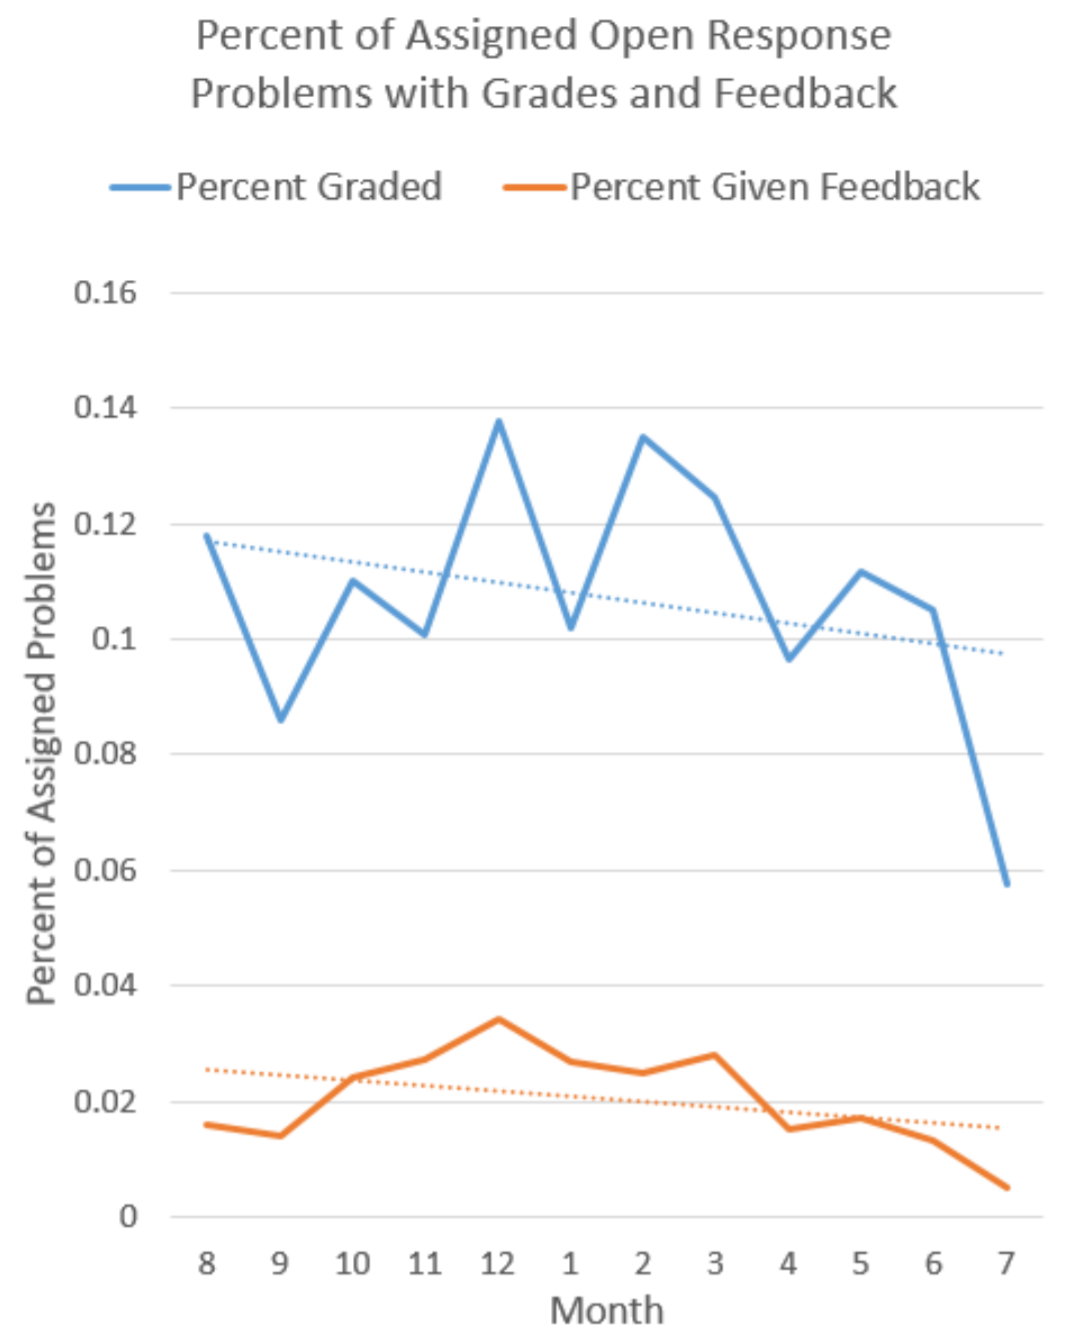
\includegraphics[width=0.5\textwidth]{images/graded_openresponse.png}
    \caption{Percent of Assigned Open Response Problems with Grades and Feedback}
    \label{img:graded_openresponse}
\end{figure}

\section{Background and Related Work}

This section describes two research projects currently in development at ASSISTments: QUICK-Comments and LIVE-CHART. The common thread in this thesis work is the development of tools to aid teachers in providing their students with more frequent feedback. These tools are built with the intention of supporting feedback creation in these larger research projects. In QUICK-Comments, the feedback takes the form of natural language message recommendations for open response mathematics questions. In LIVE-CHART, the method of feedback can take many forms, and we create detectors of student behavior to indicate to teachers the kind of feedback that might be appropriate to give to a student at a certain point in time.

\subsection{QUICK-Comments}

With the motivation of wanting to provide teachers better support while grading, and with the knowledge of the difficulties of grading open response questions, the ASSISTments research team began to work on QUICK-Comments. The goal of the QUICK-Comments project is to create a human-in-the-loop AI tool that leverages state of the art NLP to help give feedback for mathematics open response questions \cite{quick_comments_nth}. The key is to keep teachers in the driver's seat and provide them with a tool to make the feedback process easier. Figure \ref{img:quick_comments_new} shows the QUICK-Comments interface.

\begin{figure}[ht] 
    \centering
    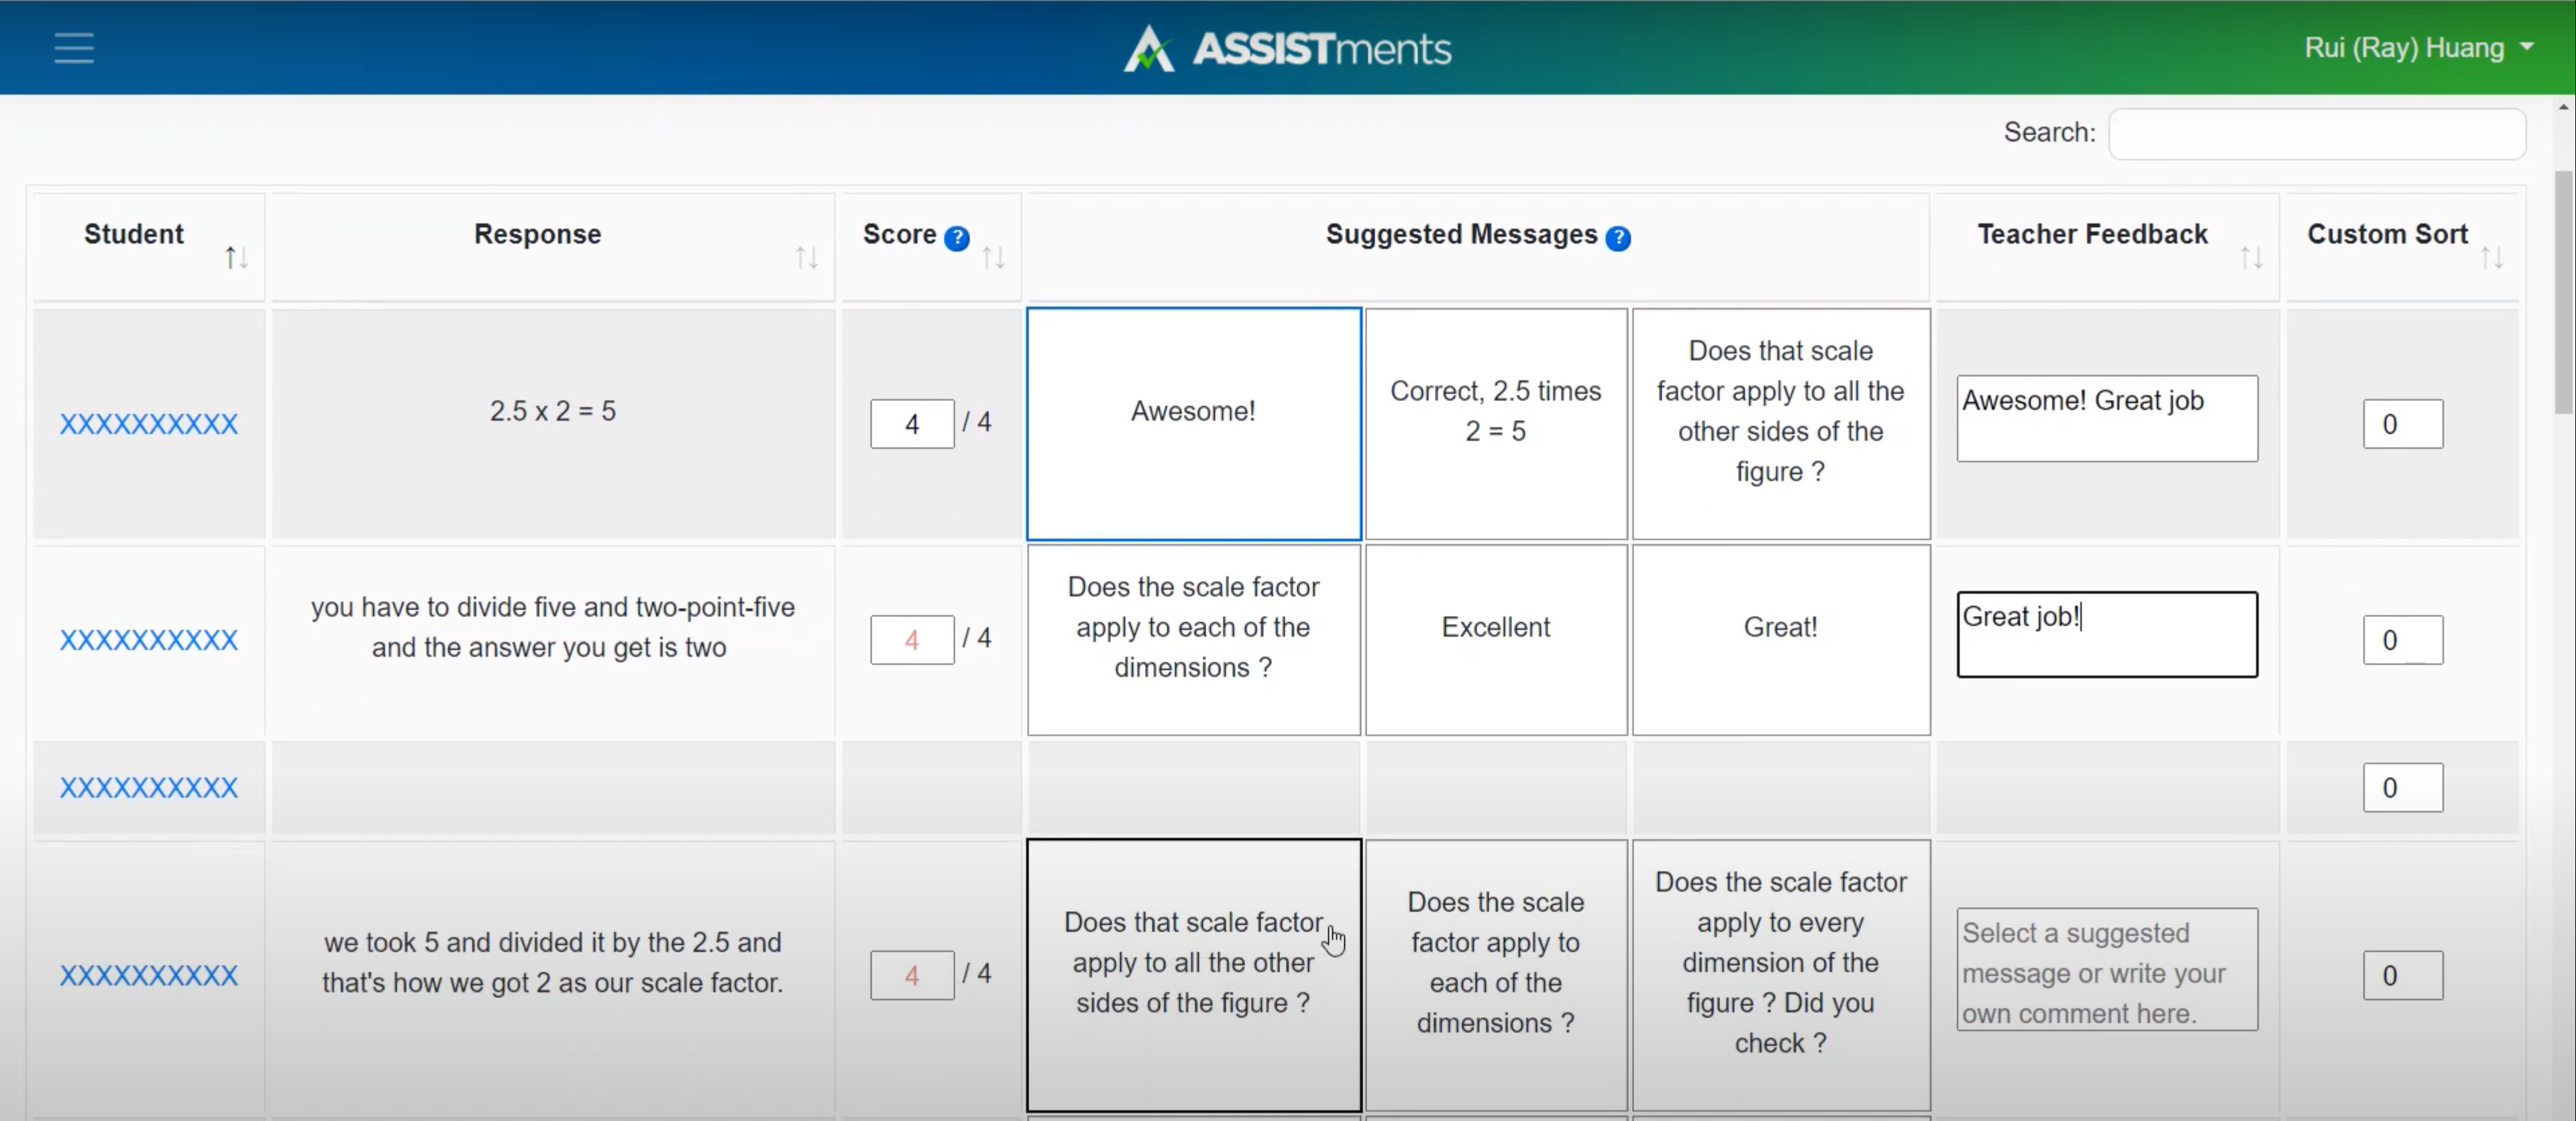
\includegraphics[width=\textwidth]{images/quick_comments_new.png}
    \caption{QUICK-Comments interface with 3 suggested comments}
    \label{img:quick_comments_new}
\end{figure}

Using the QUICK-Comments interface, a teacher can go through all the student responses submitted for a problem and they receive a suggested numeric score along with three suggested feedback messages for each one. These suggestions are based on how other teachers have evaluated the same problem. Suggestions are never sent to students without the teacher first clicking on it, and modifying it if necessary. Modifying the suggested score will also prompt the tool to change the recommended feedback messages accordingly. For example, if the tool recommends a score of 4, it will also tend to recommend short, positive messages that reflect that the answer deserves full credit. If the teacher decides to change the score to a 3, the QUICK-Comments system will now update with more critical feedback.

\subsection{LIVE-CHART}

LIVE-CHART is a set of real-time awareness tools that will help teachers better manage their students in the classroom. The teacher will be able to see where their students are as they work on a problem set and get notified when students are doing well or need help. From the viewpoint of the student, the tool allows them to discreetly signal to the teacher if they need help without having to physically indicate it. 

The tool has straightforward applications in a remote classroom setting, but it could also be beneficial for in-person settings. Just as the Lumilo tool \cite{Holstein2018StudentLB} leverages mixed-reality to augment a teacher's ability to pay attention to the students that need the most help, we hope to show a similar result with mobile and web-based versions of LIVE-CHART. A sample interface for LIVE-CHART can be seen in figure \ref{img:live_chart}. In this view, the teacher can see each of their students making their way through a problem set and their performance on the last 5 problems. If the student is struggling, their icon lights up red and they get placed in the `Requires Attention' list. If the student is progressing fine, their icon lights up green and they are put in the `Students Doing Well' list.

\begin{figure}[ht] 
    \centering
    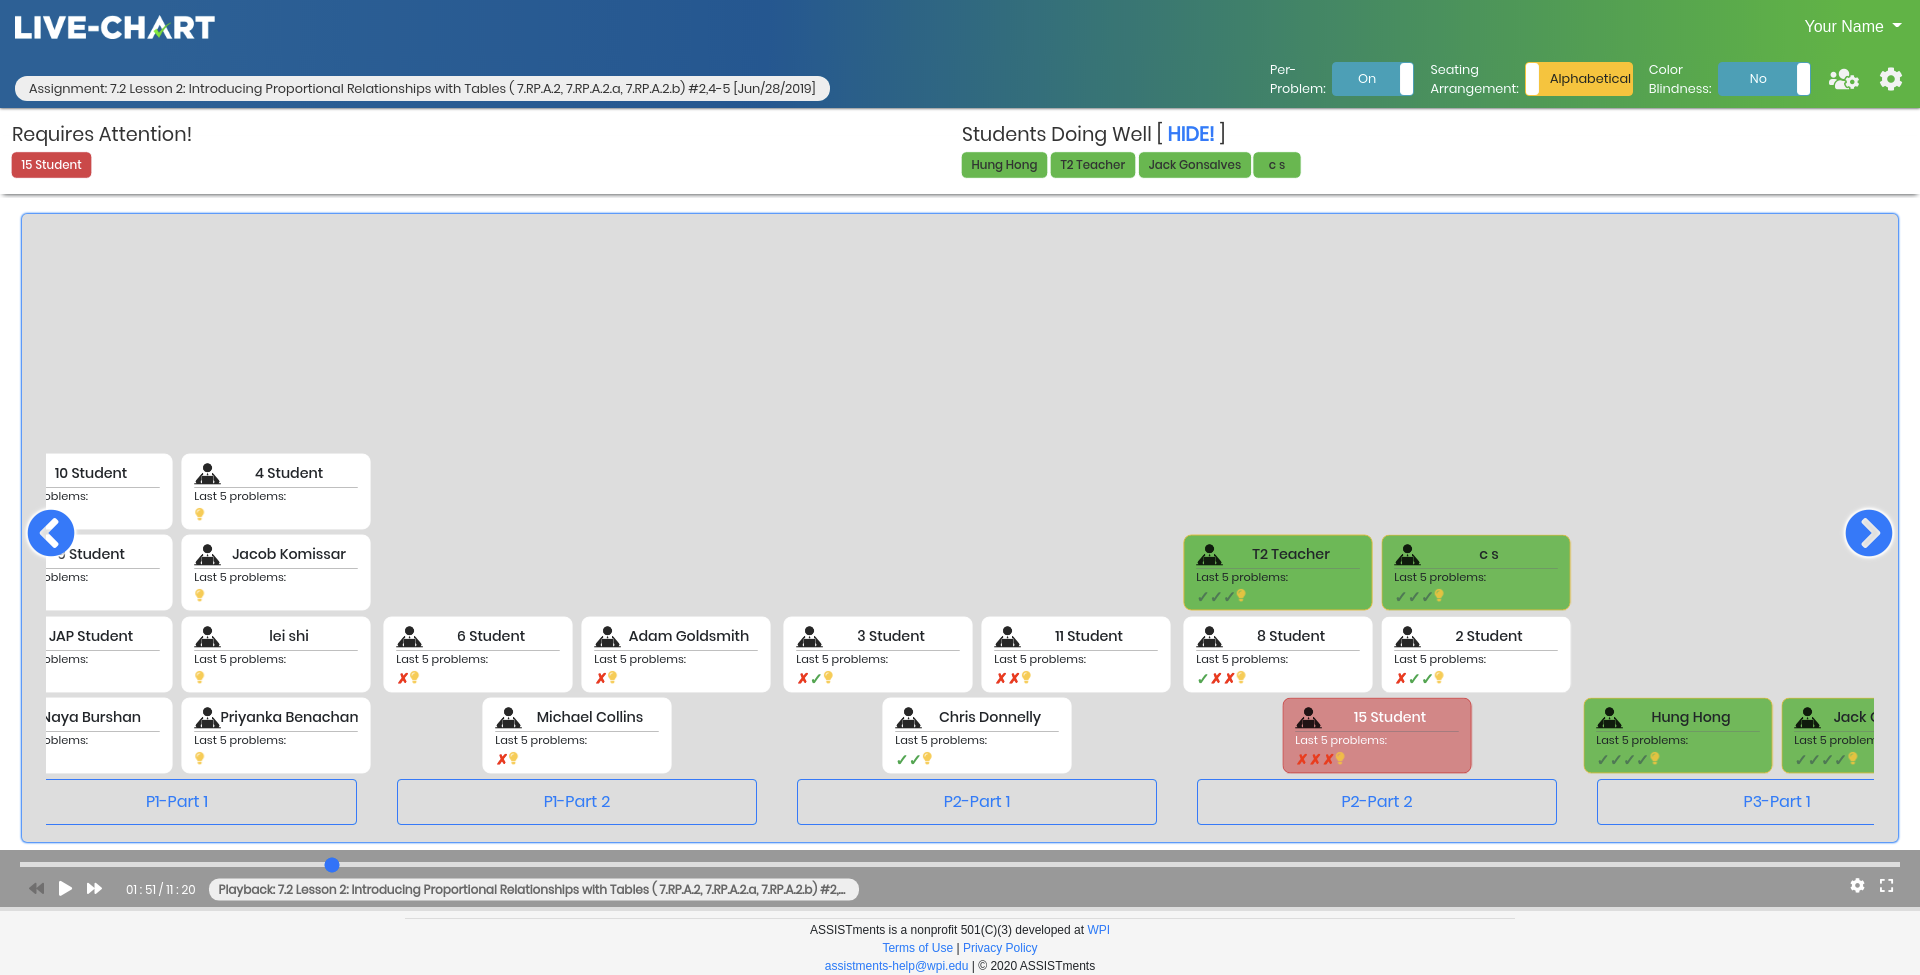
\includegraphics[width=\textwidth]{images/live_chart.png}
    \caption{Problem view of the LIVE-CHART system}
    \label{img:live_chart}
\end{figure}

\chapter{Evaluating NLP-based Feedback Models}

Our previous work has been focused on creating methods and infrastructure to evaluate the performance of feedback systems that are based on natural language generation. The first piece towards achieving this is the creation of evaluation metrics to measure our recommendation performance. The second is the infrastructure to run randomized controlled trials (RCTs). 

\section{Evaluating Comment Suggestions}

In order to evaluate a particular recommendation policy, we needed a metric that would represent a good suggestion. To create this, we used a dataset of student answers where multiple teachers graded each student answer. The metric we constructed is a measure of the overlap between different teacher comments for a single answer. We call it the Teacher Agreement Score (TAS). 

Taking a particular student answer, we find the top $R$ similar answers using our recommendation policy. We then do a one-to-one comparison across the $T$ teacher categories for each similar answer and find the average co-occurrence. We then average this value over the $R$ similar answers. Equation \ref{eq:tas} describes calculating TAS of a single student answer.

\begin{equation} 
    TAS_{i}=\frac{1}{R}\sum_{j=1}^{R}\frac{1}{T}\sum_{t=1}^{T}int(Category_{i,t}=Category_{j,t}) 
    \label{eq:tas}
\end{equation}

In the example in image \ref{img:tas_example}, $R = 3$ and $T = 4$. We are calculating the TAS for the student answer ``no because the 50 and 10 amt the same3" with 3 similar answers and 4 teacher categories.

\begin{figure}[ht] 
    \centering
    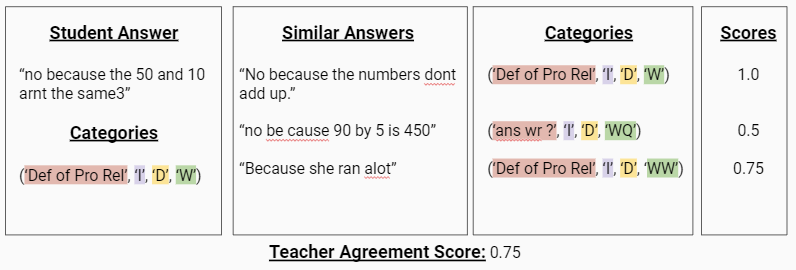
\includegraphics[width=\textwidth]{images/tas_example.png}
    \caption{Calculating the Teacher Agreement Score (TAS) for a student answer}
    \label{img:tas_example}
\end{figure}

Once we have calculated the TAS for a particular answer, we go through all the answers and repeat the calculation in a hold-one-out manner (holding out the answer and finding the top $R$ most similar answers). Averaging across all the answers, we get the TAS for a particular problem. Repeating the process across all the problems gives us an overall TAS for the recommendation policy. We use both the per-problem TAS and overall TAS to compare recommendation policies.

This work was done in collaboration with John Erickson, Taylor Stefovic, Priyanka Benachamardi and others, and went into a broader analysis of combinations of sentence representation methods and distance metrics to compare recommendation policies.

\section{RCT Infrastructure for QUICK-Comments}

Randomized Controlled Trials (RCTs) or A/B Tests are an important method to iteratively improve software. The main idea is to randomly assign users into two groups: control and treatment. The treatment group is shown the new feature being studied while the control group is given the `business as usual' condition. In order to support RCTs for QUICK-Comments, software components and data tables had to be designed. 

The overall flow of data through the QUICK-Comments tool is shown in figure \ref{img:rct_overview}. The green RCT layer is the new component we designed and it represents the functions and database tables that handle the randomization and data logging. The detailed ERD for the database tables can be found in the appendix.

\begin{figure}[ht] 
    \centering
    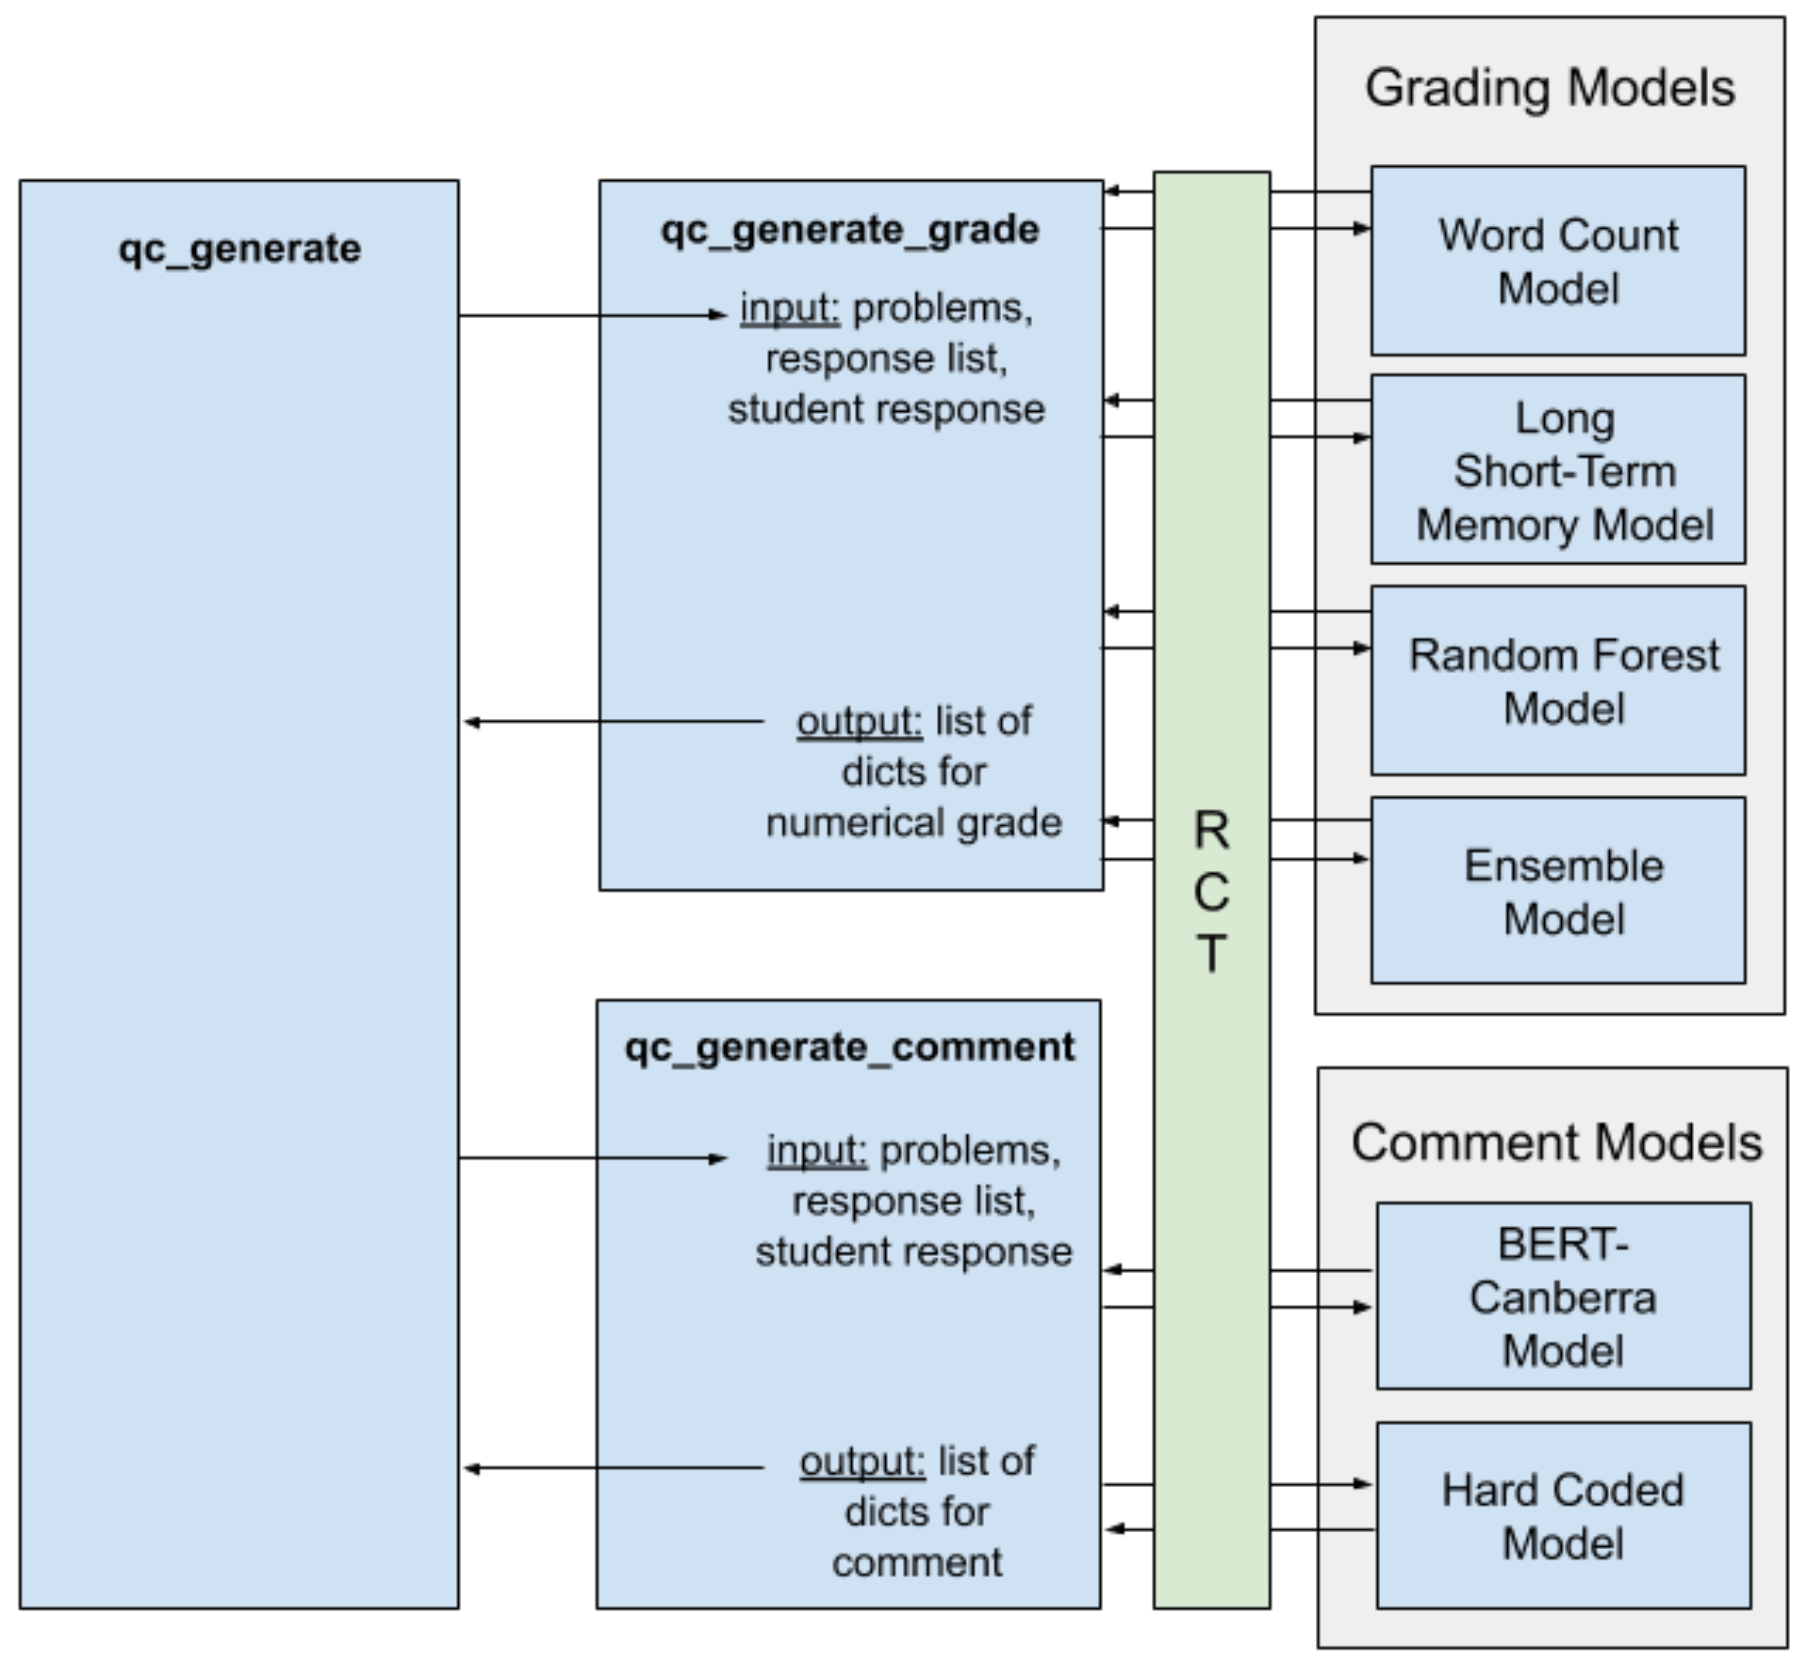
\includegraphics[width=0.6\textwidth]{images/rct_overview.png}
    \caption{RCT infrastructure design for QUICK-Comments}
    \label{img:rct_overview}
\end{figure}

In order to generate feedback comments, the QUICK-Comments tool makes use of 2 kinds of models: grading models and comment models. Since the quality of an answer (as measured by the grade) predicts the kind of comment that is appropriate, we first generate a predicted grade and use that as a feature in our comment generation.  

The new RCT layer of the QUICK-Comments tool fits between the function calls to generate comments and the trained models. With this layer, researchers will have the ability to randomize which models are used based on the given user conditions to test out different comment generation strategies. There can be three different levels of user condition randomization. An experiment can be randomized on the teacher, teacher-assignment, or teacher-assignment-student level. These three possibilities for randomization are based on the identification numbers of the user or the assignment.

This work was done in collaboration with Sami Baral and Kirsten Hart and has since been built upon by Priyanka Benachamardi for her thesis work.

\chapter{Activity Detectors for Problem-Solving Action Data}
The focus of QUICK-Comments is using NLP to generate and suggest feedback messages to students' open responses in mathematics. But there are other areas that we can provide feedback to students by leveraging the data logged as they work on ASSISTments and solve their homework. Feedback can be more than just based on the final answer a student reaches. We believe that there is a lot we can do to help students by providing them feedback on their approach to solving problems as they do their homework.

Our current work expands feedback generation to student actions. The objective of this work is to make it easier for teachers to leave feedback and increase the amount of feedback that students receive. The key differences in this work are the training data and the form that the feedback takes. In this case, what we are training on is student action data - a series of timestamped actions. We are using this data to create detectors of feedback which can be reported to the teacher. The teacher can use the output of these detectors to give feedback to students. If these detectors are integrated with LIVE-CHART, the feedback takes the form of live conversations or text messages.

\section{Dataset and pre-processing}
This data was collected by showing teachers a snippet of student actions and having them tag the behavior they observed the student exhibiting. Student actions are timestamped interactions that a student makes with the ASSISTments platform as they solve problems (e.g. `Submitted a response', `Requested the answer', `Finished problem'). The teachers select the series of timestamps they are commenting on and leave a comment and comment category. Figure \ref{img:qc_action} shows an example of the screen the teachers saw as we performed this data collection. 

\begin{figure}[ht]
    \centering
    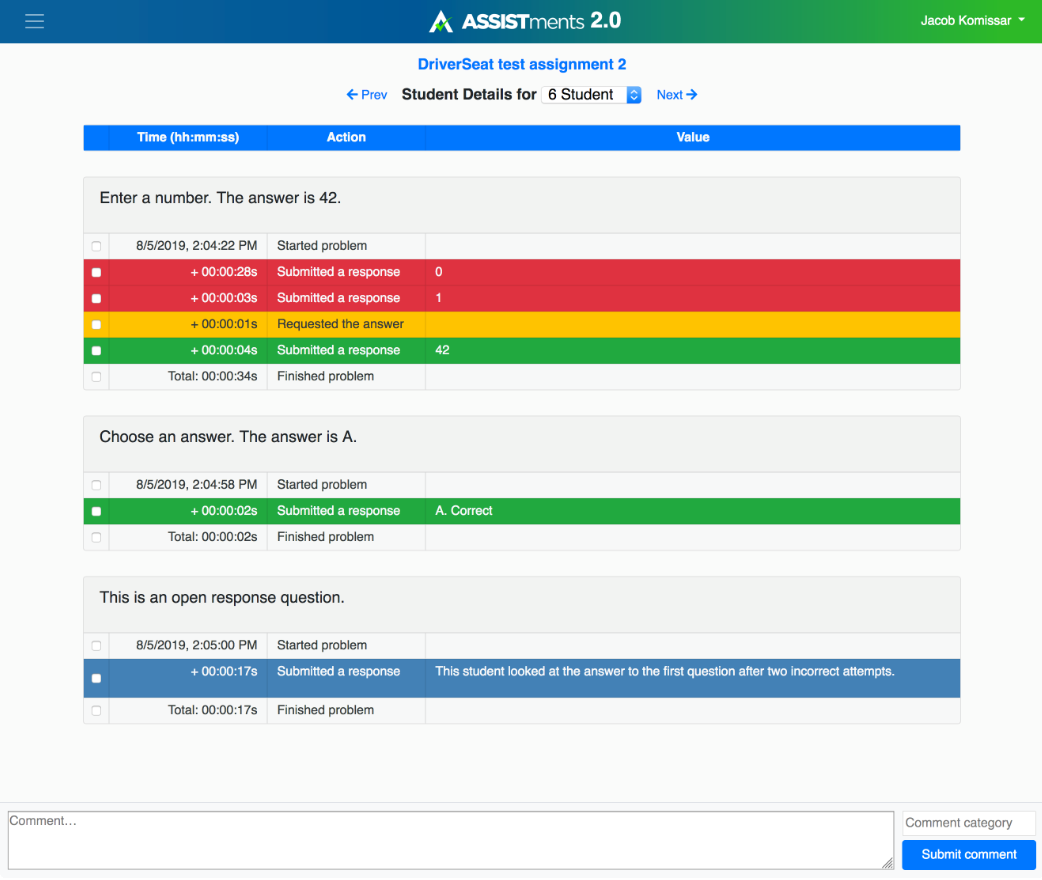
\includegraphics[width=0.8\textwidth]{images/qc_action.png}
    \caption{Feedback comments for student actions}
    \label{img:qc_action}
\end{figure}

A significant amount of work for this project went into cleaning the data and pre-processing it to create our model. In addition to this, some pre-processing steps were needed so that we were following previous work and doing a student-level evaluation ensuring that we weren't learning from and predicting on the same student. The following subsections describe the pre-processing steps taken.

\subsection{Feature Creation}
Each action in ASSISTments is given an action name. Some examples of these are `AnswerRequestedAction', `HintRequestedAction', `ProblemFinishedAction'. Each action name was merged with the answer correctness. When the action had no answer correctness, it would be blank, otherwise it would have a true or false appended to the name. For our first model, we had 28 features: 27 features were the one-hot-encoded action name and answer correctness combination, and one feature indicated the seconds since last action.

Some possible features that can be used in the future are the answer text and the problem type. The problem type will need to be found in the ASSISTments database. For the text feature, there will need to be an embedding step. We would expect to see that \texttt{answer\_text} correlates with answer correctness if we have NLP models trained per problem to learn which phrases score the most points.

\subsection{Maintaining Student Sequences Within Fold}
When testing out our model, we decided to perform cross-validation. Following similar work on affect detection \cite{affect_detection}\cite{Wang2015TowardsBA}, we wanted to distribute students across the folds to create 10 roughly equal-sized groups and perform a student-level cross validation. Due to the nature of the data where different students have different action sequences, this means that the data within folds won't be exactly equal - but there won't be large disparities when looking at large numbers of students.

\subsection{Collapsing Categories} 
Since teachers were free to leave their own comments and create their own comment categories as they saw fit, there is overlap between categories of different teachers with slight differences. One of the things we explored was ways to collapse these categories in order to create labels that we could predict across teachers.

We took a few approaches to this, ranging from hand-coding the categories to exploring word embeddings. However, these techniques are reliant on semantic similarity and since we did not have a measure of inter-rater reliability, we could not use it. In order to collapse categories effectively, we would need to have multiple teachers grade the same responses so that we have a measure of agreement across teachers. Once we have a model that is built for predictions across teachers, we can use the embedding layer to find which categories overlap in an unsupervised manner (such as clustering). This would give us a method of condensing down the categories in a way that does not rely on semantics.  % TODO: check with anthony

% \subsection{Data Cleaning and Formatting}

\section{First Model: When to give Feedback?}
The first model created, takes in a series of student actions and outputs a binary prediction of which actions the teacher left feedback for. Essentially, the model attempts to flag which actions taken by a student are noteworthy. 

Since LSTMs are good models for time series and useful for modelling sequences that may have lags between timesteps that are significant, we thought it would be suitable to apply here. When teachers select a sequence of actions to comment on, we do not know which parts of the sequence contain information that is more significant. We hope that in the aggregate, this information can be learned. 

We implemented the lstm model using the Keras API for TensorFlow. We created a sequential model that had an lstm layer with 50 hidden unites and a dense output layer with sigmoid activation. The model was trained for 200 epochs with early stopping and a patience of 10. This usually caused training to stop after 30 epochs, and plotting the validation loss indicated that this was around optimal. As described earlier, the model was fit and evaluated 10 times to do a 10-fold cross validation.

All code for this work can be found at \href{https://github.com/aaron-alphonsus/student-actions}{github.com/aaron-alphonsus/student-actions}. This repo only contains code - any data that was used will have to be requested from the ASSISTments research team: \href{http://www.assistmentstestbed.org/faq}{www.assistmentstestbed.org/faq}.

\section{Second Model: Detecting Positive Feedback}
In our second model, we had two goals we wanted to meet. The first was that we wanted to be able to create something that could be applied to the infrastructure already in ASSISTments. LIVE-CHART was identified as a potential candidate for this. With that in mind, we began to look at the data to pick out a potential behavior that we thought would be interesting to detect. We also needed to keep in mind that there needed to be a decent number of these instances present. 

From the literature, we noticed that studying positive feedback could be an interesting angle to approach this as it wasn't focused on as much as critical feedback. Looking at the data, we picked out the teacher that had graded the most problems and chose one of their categories as our behavior of interest. This ended up being the category `Thoughtful self correcting'. In all, this teacher had 27 different categories. 1177 actions were flagged and marked with `Thoughtful self correcting'. The vast majority of the actions were not commented on (150430 actions)

Once again, our implementation was an lstm model using Keras. The architecture and training method was the same as our previous approach. This time however, the model tended to train for 70-80 epochs before early stopping. The evaluation of the model was done the same way, using a student-level 10-fold cross validation.

%TODO top categories graphic
%TODO plot model?

\section{Results}

Both models were evaluated by performing 10-fold cross validation, being careful to maintain student sequences within a fold. AUC and RMSE were calculated for each fold and averaged across folds. The first model achieved an AUC = 0.602 and RMSE = 0.298. The results of the second model that detects positive behavior was slightly better, achieving an AUC = 0.645 and RMSE = 0.161. To contextualize these results, we look to affect detection and the work done by Ocumpaugh et al. \cite{affect_detection} and Wang et al. \cite{Wang2015TowardsBA}. These were some of the first attempts to create detectors of affect, and the AUC achieved is comparable. However, both of these works use many more features than we do (69 and 232 respectively) and feature engineering could be an area to improve on in our work (e.g. a feature indicating the type of question - true/false, multiple choice, open text)
% For example, an auc of 0.65 would indicate that a detector of boredom can distinguish a bored student from a non-bored student 65% of the time. 

\chapter{Discussion}

In this work we extend our work on feedback to a dataset of student actions. We created models for the sequence to sequence tasks of 1) detecting when teachers give feedback and 2) detecting a particular positive behavior within the student actions. These detectors can be applied to student reports to flag rows of student actions where students could receive feedback. Since this data was collected from other expert teachers, our predictions are an indication of what a teacher would find notable for comment.

Our next steps would be to examine how categories overlap across teachers so that we can not only predict where we can give feedback but also what category of feedback. In order to do this, we need to find some measure of agreement across teacher categories. This was a simpler task in our previous work as multiple teachers had graded a single problem set so we could just look at a particular student answer and count the co-occurrence of categories from different teachers. In this case, since teachers only graded their own students, we need to come up with a different way to cluster and collapse categories so that we can predict them.

By creating the detector of positive feedback, we have the goal of detecting when student actions exhibit positive behavior. This detector can be used to analyze simple timestamped action data to detect the presence of the behavior `Thoughtful self correcting'. With tweaks to the model, we can build towards a detector that could be deployed for a real-time setting like LIVE-CHART. To do this, we will need to modify the output so that it makes a prediction only for the final timestep in the sequence, instead of a prediction for the entire sequence.

\clearpage

% \section{First Section.}
% More Text.
% \subsection[Alternative title for the Table of Contents]{First Subsection.}
% Even more text, maybe a formula:
% \begin{equation}
% \sum_{i=1}^{n}i=\frac{n(n+1)}{2} % much easier than Microsoft Equation
%                                  % Editor :)
% \end{equation}
% \subsubsection{First Sub-subsection.}
% This is really deep down in the hierarchy. Maybe you shouldn't even
% use sub\-subsections. It goes further down (paragraphs), but I don't
% think you'll need that\footnote{By the way: notice that, although we
% have doublespacing here, the footnotes are singlespaced. This is
% intended and good. If you want to change that, try, but this is really
% how it should be.}.

% \section{Other thoughts.}
% Okay, what else? \cite{10.1145/2342441.2342467}
% Let me quickly put a figure here, maybe a piece of pseudo code.
% That way, you can see how this is done. It's a little painful, but
% looks really cool. We will call it Figure~\ref{fig:source_algo1}. The
% numbering is automatic---don't worry about it.

% %First, we want to make our life easier and define a ``TAB'' command.
% \newcommand{\T}{\hspace*{5mm}}

% % Start a figure
% \begin{figure}[htb]
% % We would like to have the whole thing in the center of the page
% \begin{center}
% % We want a frame. 
%   \fbox{
% % The figure should autoformat to half the page width
%       \begin{minipage}{0.5\textwidth}
% % Now comes the content.
% % For source code, you have to leave an empty line after each line of
% % code.
% % Note that this is text-mode, that's why all formluae are typeset in
% % math-mode (enclosed in dollar-signs $a+b$)
% % Each line needs a font command a la \texttt{}, \textsc{}, textbf{}
% % You could use \begin{verbatim}\end{verbatim} for source code, but then 
% % you can't do any more formatting in you source file. May be appropriate
% % sometimes. 

% \textsc{Bellman-Ford} $(G,w,s)$

% (1) \textsc{Initialize-Single-Source}$(G,s)$

% (2) \textbf{for} $i\leftarrow 1$ \textbf{to} $|V[G]|-1$ \textbf{do}

% (3) \T\textbf{for} each edge $(u,v)\in E[G]$

% \T\T\T\textbf{do} \textsc{Relax} $(u,v,w)$

% (4) \textbf{for} each edge $(u,v) \in E[G]$

% \T\T \textbf{do if} $d[v]>d[u]+w(u,v)$

% \T\T\T \textbf{then return} \textsc{false}

% (5) \textbf{return} \textsc{true}

% % End of content, closure of minipage, frame, and centering.
%       \end{minipage}
%   }
% \end{center}
% % Caption
% \caption{This is a very simple algorithm in pseudocode.}
% % A label to refer to the figure.
% \label{fig:source_algo1}
% % End of figure
% \end{figure}

% \noindent
% And so on, and so on.

% Please remember that you have to compile a document several times when
% you did changes that affect figures, table of contents, bibliography,
% etc. (This is always the case if you get the warning: ``LaTeX Warning:
% Label(s) may have changed. Rerun to get cross-references right.'').

% The recommended sequence is :

% \texttt{latex foo.tex}

% \texttt{bibtex foo}

% \texttt{latex foo.tex}

% \texttt{latex foo.tex}

% Let's assume this is the end of your thesis text.

% Now come appendices, if you had any.
% Appendices are automatically numbered, just like everything else in
% LaTeX. But only after you gave this command
\appendix

% \chapter{More to say}

\chapter{ERD for QUICK-Comments RCTs}
\begin{figure}[ht] 
    \centering
    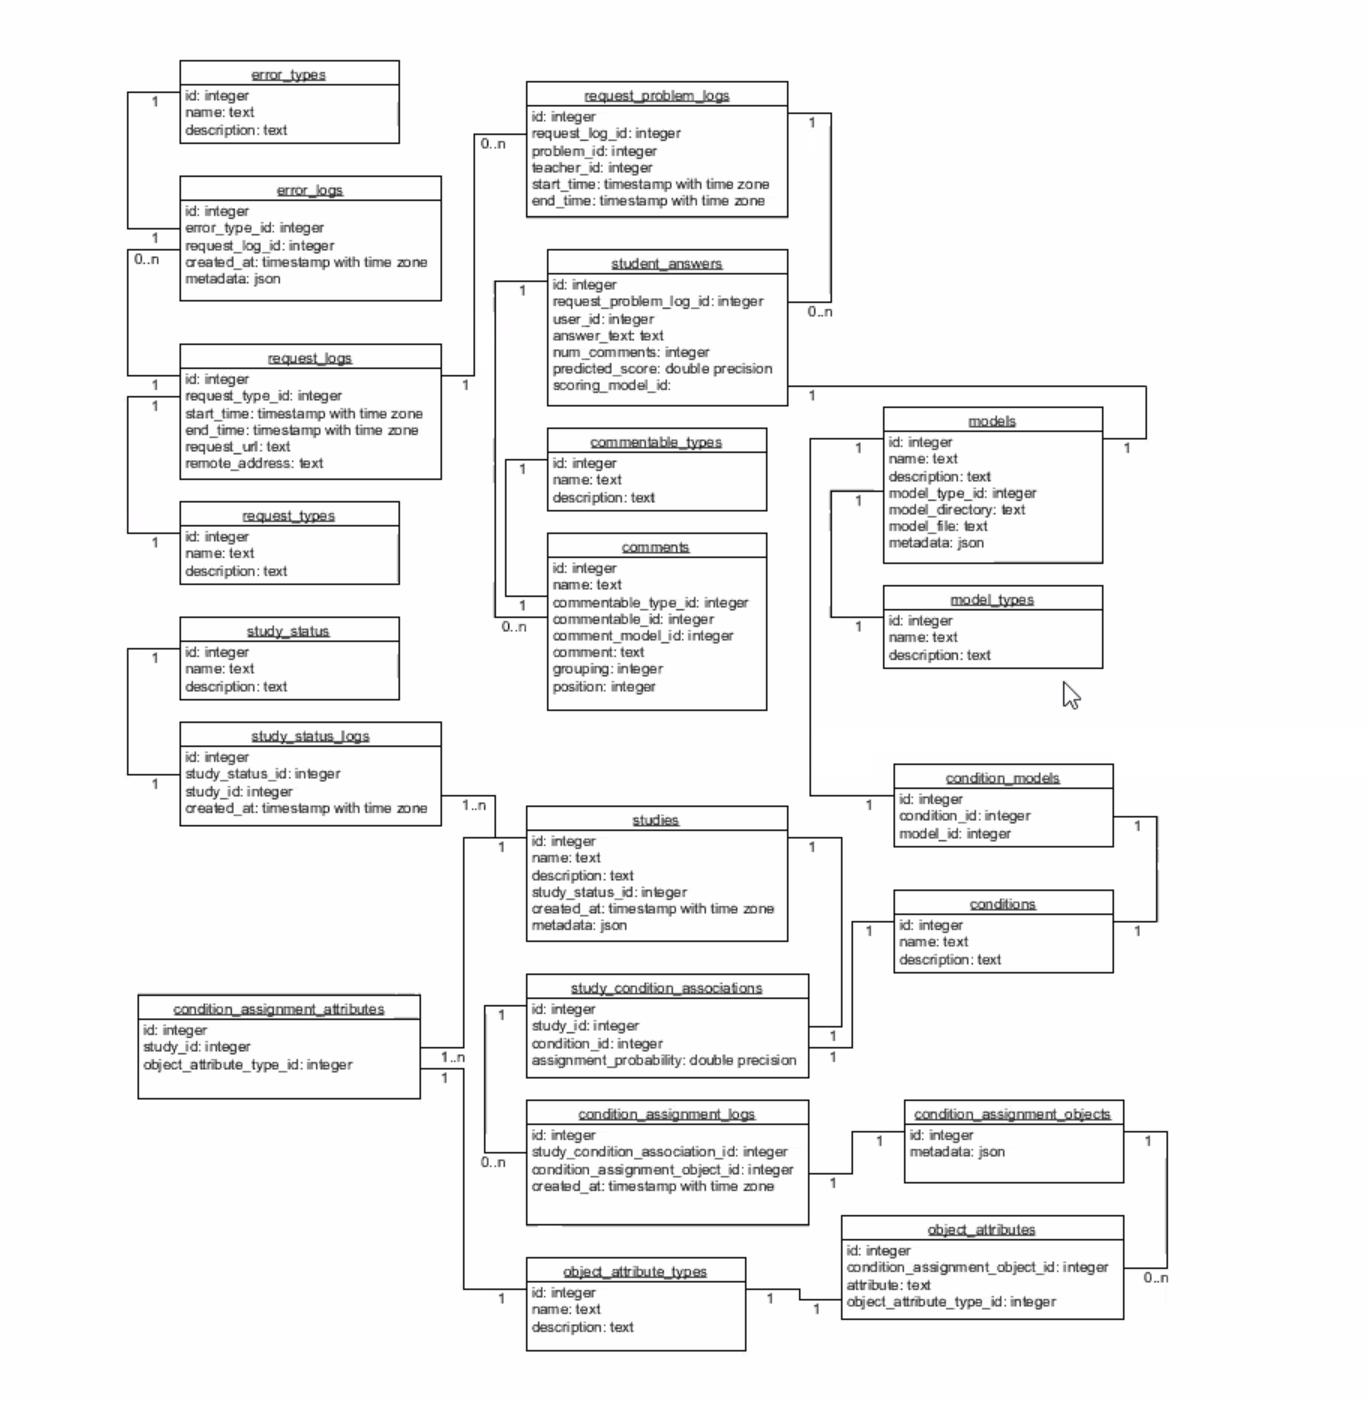
\includegraphics[width=0.85\textwidth]{images/erd.png}
    % \caption{}
    \label{img:erd}
\end{figure}


% Last and least (at least, that's what the library says) - the
% Bibliography.

% you can save some space by having the bibliography singlespaced, if you want
% \singlespacing

% You should become familiar with the BibTeX program, which
% uses a *.bib-file to collect all citations that you have. It's a lot
% prettier than typing all the citations right into the document. The 
% reference to citations also works well that way, but the exact 
% explanation of that will be on the CS-GSO homepage, whenever I'll ever 
% have time for that.
%
%
% If you use BibTeX, the bibliography is very easy. You refer to
% citations in the text with \cite{tag}, where tag is the tag that you
% defined in the bib-file.
% Then, you run bibtex once in a while during compilation, and the
% rest is done in two lines:


% \bibliographystyle{alpha}
% \bibliography{foo}
\printbibliography

% which assumes a file foo.bib in your working directory.
% The word ``Bibliography'' will appear in your document as soon as
% you used ``bibtex'' on the command line.
%
% For reference on this, refer to the CS-GSO homepage.

%============================
%That's all, folks. Have fun.
%
%                     Andreas
%============================


\end{document}








